\label{sec:method}

\subsection{System Architecture}

Figure~\ref{fig:arch} shows the end-to-end detection pipeline. Windows hosts in the smart
grid OT (Purdue Levels 1--2) and IT (Level 3) networks generate audit events that are
forwarded to a centralised collector. The pipeline ingests the raw event stream, groups it
into sessions by a 30-minute inactivity timeout, extracts feature vectors, and classifies
each session with a pre-trained Random Forest model.

\begin{figure}[!t]
  \centering
  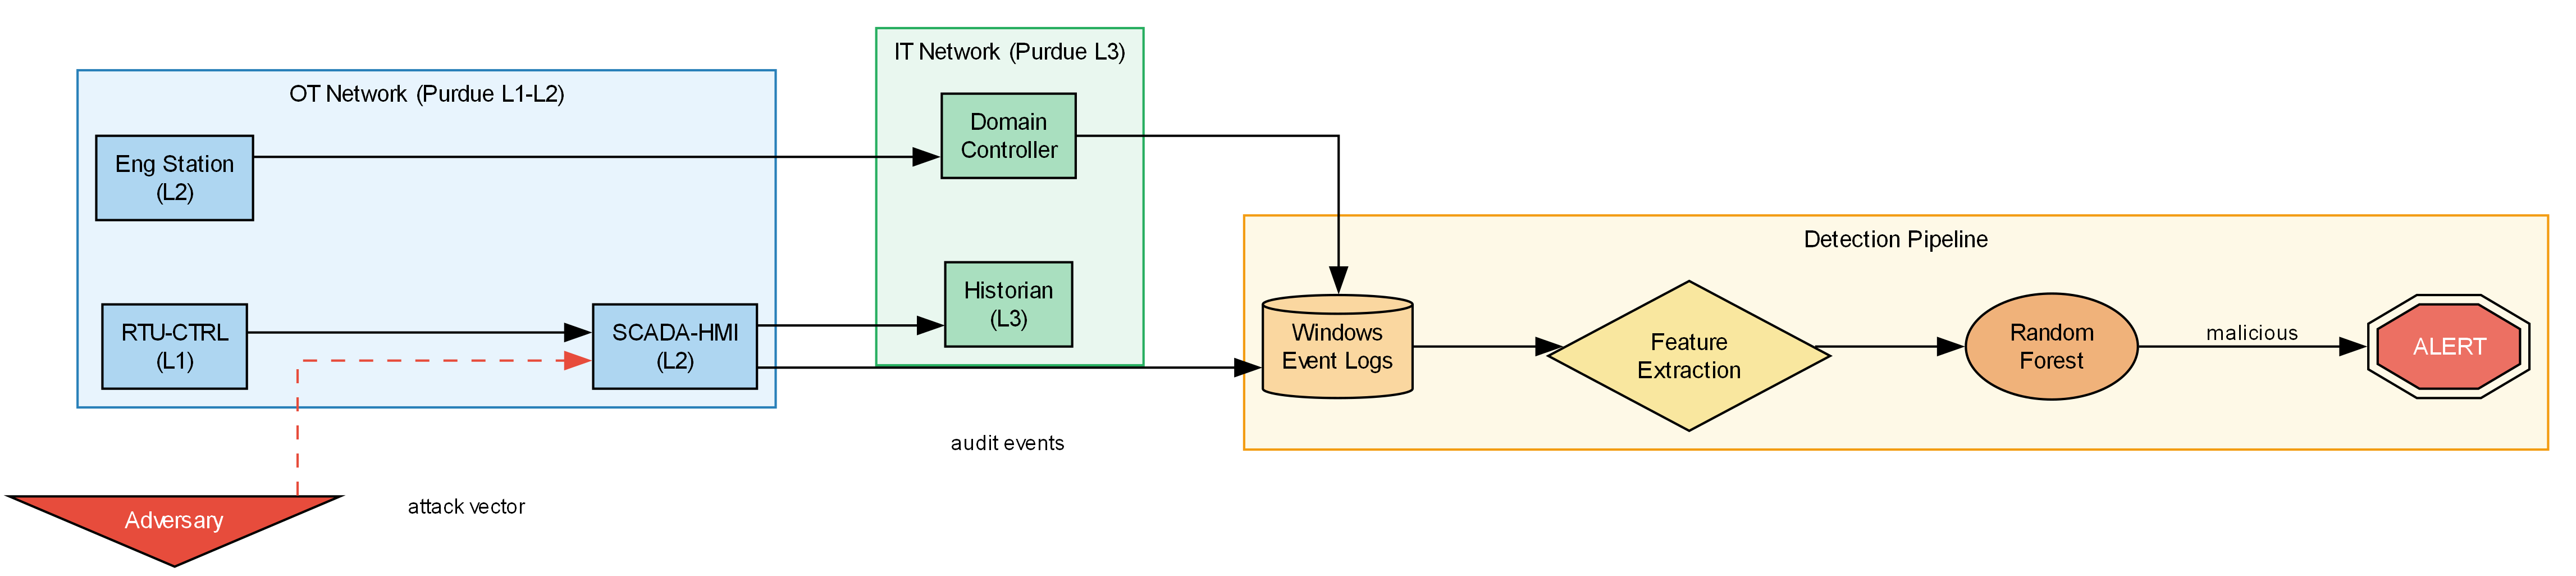
\includegraphics[width=\columnwidth]{figs/architecture.png}
  \caption{System architecture: event collection, feature extraction, and classification
           within the smart grid IT/OT hierarchy.}
  \label{fig:arch}
\end{figure}

\subsection{Synthetic Data Generation}

The generator produces structured records with fields \texttt{timestamp},
\texttt{event\_id}, \texttt{source}, \texttt{user}, \texttt{hostname},
\texttt{description}, \texttt{label} (0 = benign, 1 = malicious), and
\texttt{session\_id}. Benign sessions simulate normal operator activity: a 4624 logon event
followed by a variable-length sequence of process creations (4688/4689), object accesses
(4663/4656), and a terminal 4634 logoff. Malicious sessions implement four attack patterns:

\begin{enumerate}
  \item \textbf{Lateral movement}: 3--8 consecutive 4625 failures from an unexpected source
        IP, followed by a 4624 success, modelling credential brute-forcing.
  \item \textbf{Persistence}: event 7045 (service install) targeting a SCADA host,
        immediately followed by 7036 (service state change) and 4688 (process creation).
  \item \textbf{Privilege escalation}: 4672 (special privileges) immediately preceding
        4688 with an anomalous process name (\texttt{mimikatz.exe},
        \texttt{psexec.exe}).
  \item \textbf{Reconnaissance}: a burst of 8--20 event 4663 (object access) records
        within 30 seconds on HMI or RTU hosts.
\end{enumerate}

\subsection{Feature Engineering}

Session-level features are extracted in five groups, as illustrated in
Figure~\ref{fig:pipeline}:

\begin{figure}[!t]
  \centering
  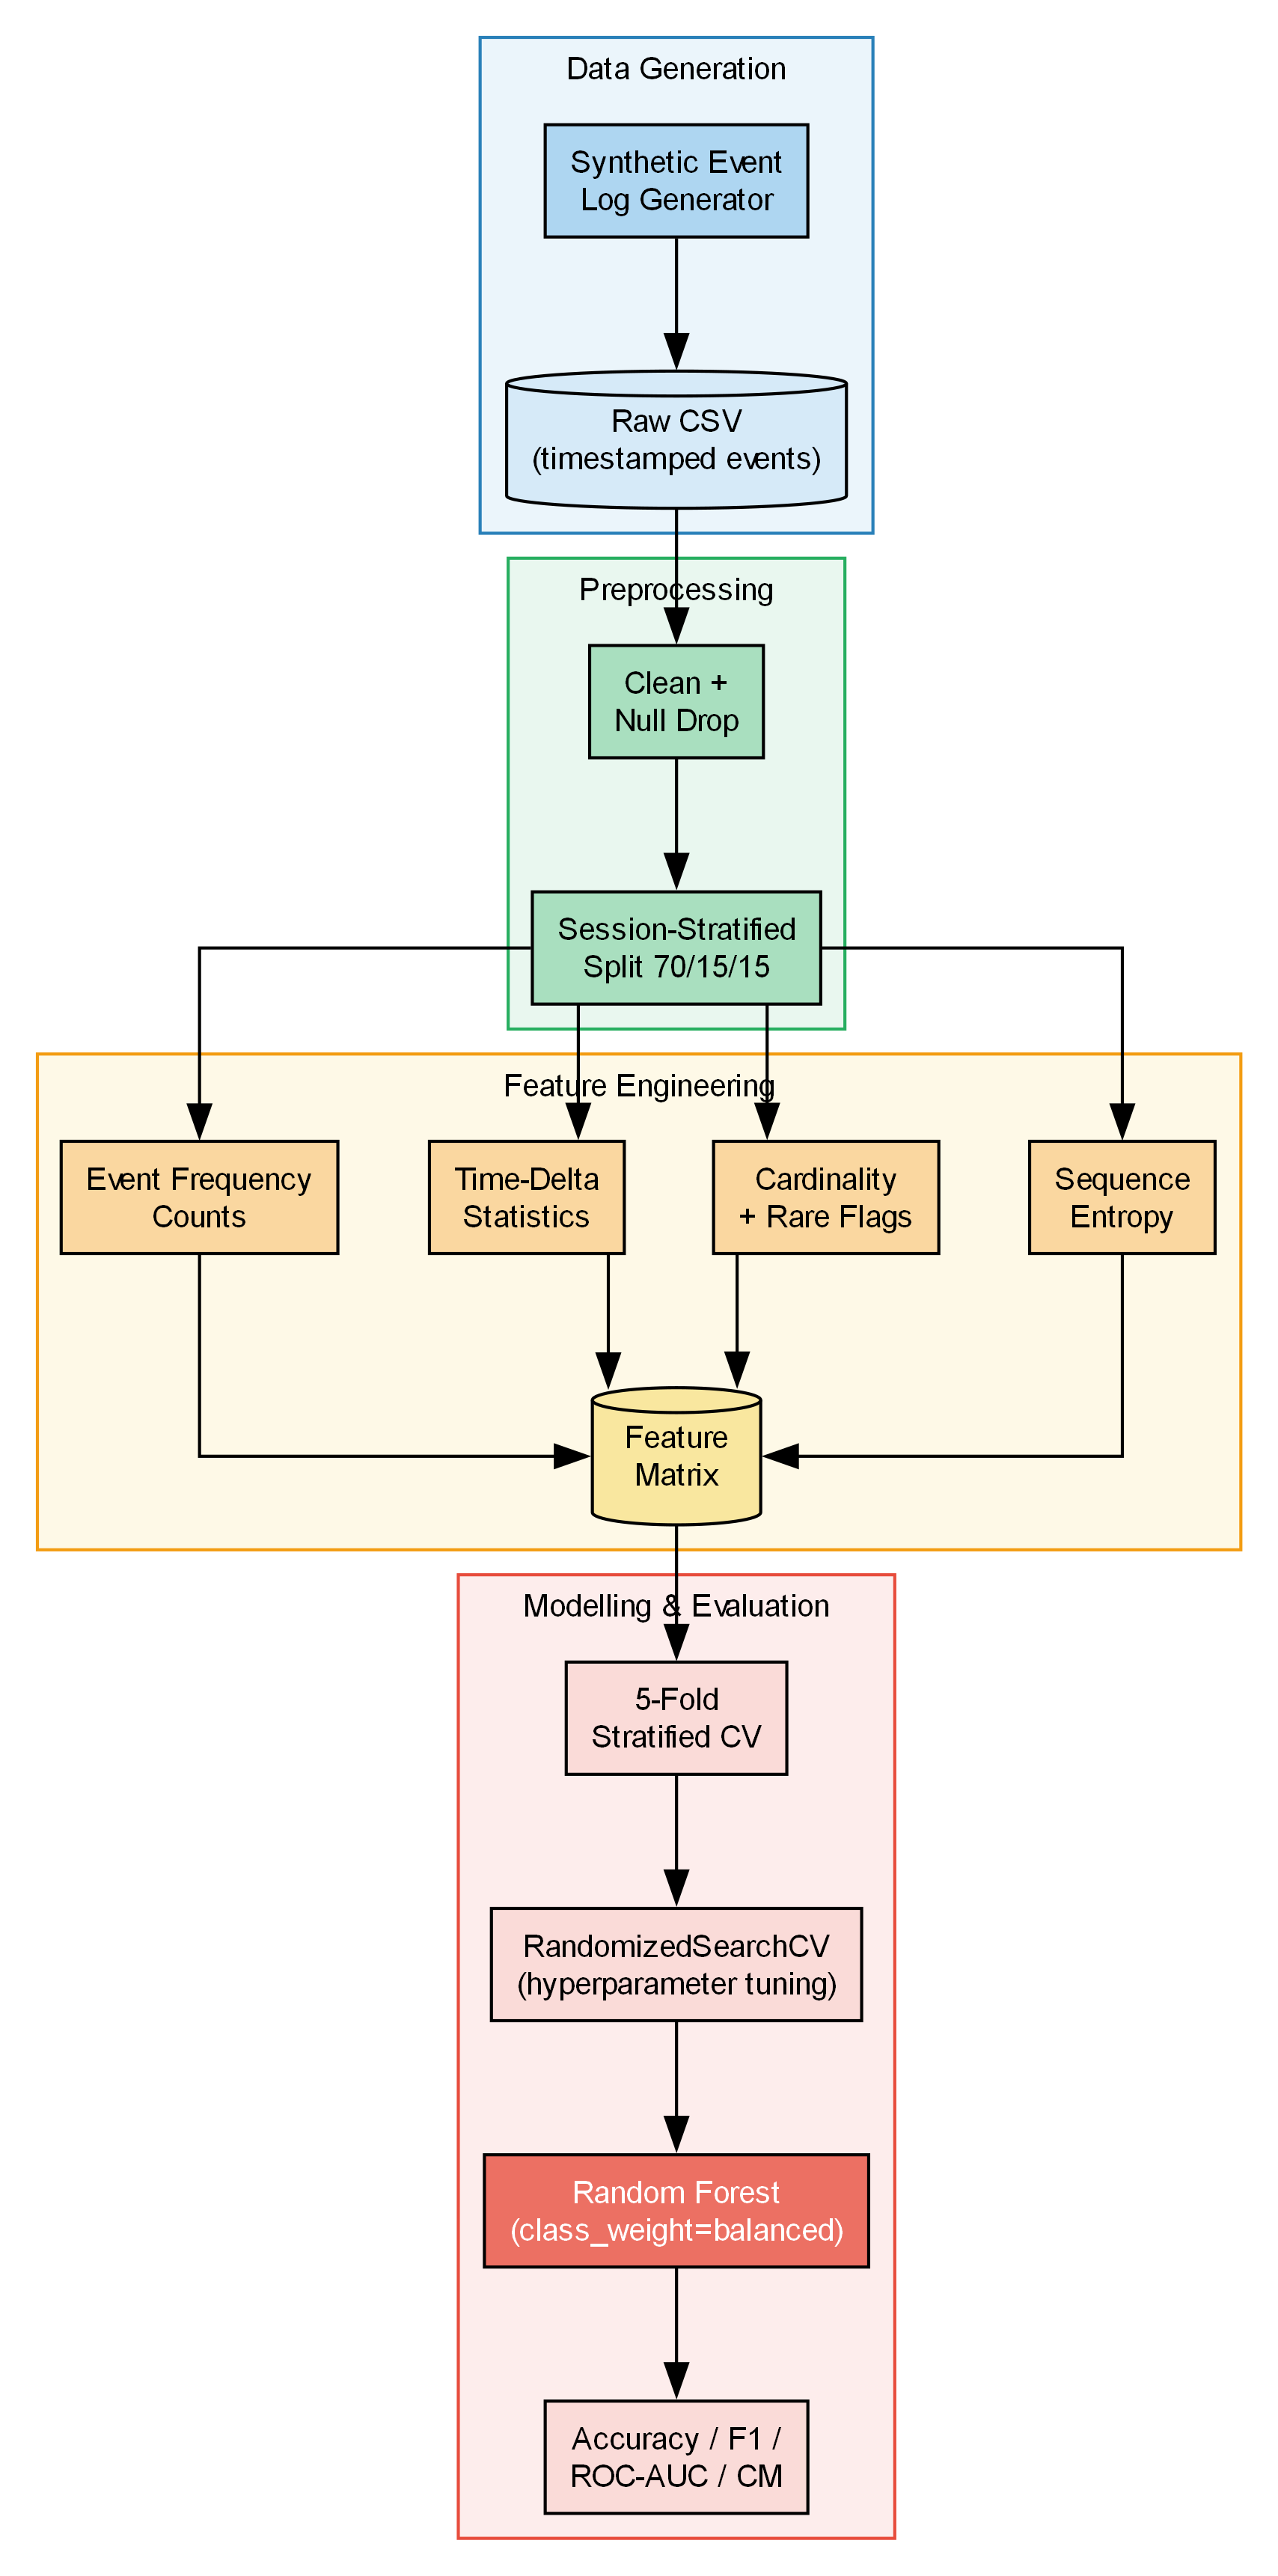
\includegraphics[width=\columnwidth]{figs/pipeline.png}
  \caption{Data pipeline: from raw event logs through feature extraction to model
           evaluation.}
  \label{fig:pipeline}
\end{figure}

\begin{enumerate}
  \item \textbf{Event frequency counts}: occurrence counts of each of 13 event IDs
        (4624, 4625, 4634, 4648, 4672, 4688, 4689, 4720, 4732, 7045, 7036, 4663, 4656)
        plus a total event count.
  \item \textbf{Time-delta statistics}: mean, standard deviation, minimum, and maximum of
        inter-event gaps (in seconds) within a session, capturing temporal burst patterns.
  \item \textbf{Host/user cardinality}: counts of unique \texttt{source}, \texttt{user},
        and \texttt{hostname} values, indicating lateral spread.
  \item \textbf{Rare-event flags}: binary indicators for event IDs appearing in fewer
        than 5\% of benign training sessions.
  \item \textbf{Sequence entropy}: Shannon entropy $H = -\sum p_i \log_2 p_i$ over the
        empirical distribution of event IDs within a session, capturing randomness in
        attacker behaviour.
\end{enumerate}

\subsection{Model and Evaluation Protocol}

We select Random Forest \cite{breiman2001} as the primary classifier. Its tree-ensemble
structure handles heterogeneous feature scales without normalisation, the
\texttt{class\_weight=balanced} setting compensates for the $5:1$ benign/malicious ratio
without oversampling, and feature importance scores provide academic interpretability.
Hyperparameters (\texttt{n\_estimators}, \texttt{max\_depth}, \texttt{min\_samples\_split},
\texttt{max\_features}) are tuned via \texttt{RandomizedSearchCV} with 20 iterations over
specified grids. The evaluation protocol uses 5-fold stratified cross-validation on the
training set, with final performance reported on a held-out test partition (15\% of
sessions). Metrics: accuracy, precision, recall, macro and per-class F1, ROC-AUC, and
confusion matrix.
